\section{Network Scenario}
\label{sec:NetworkScenario}
\begin{figure}
\begin{center}
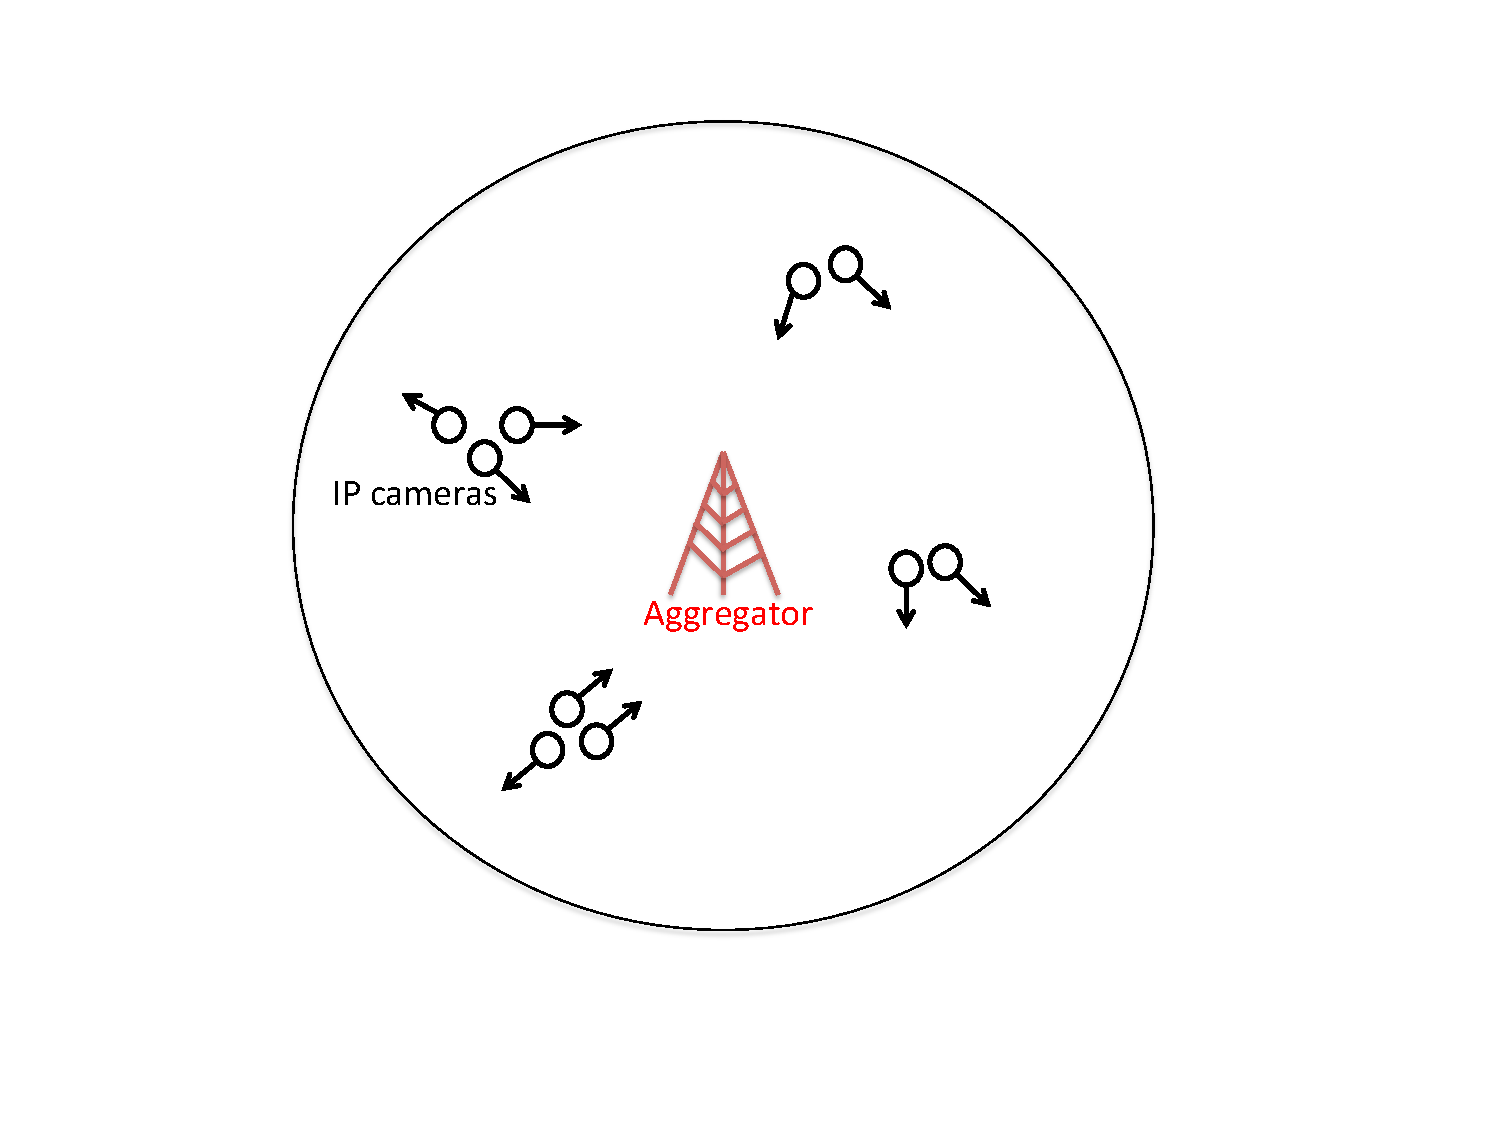
\includegraphics[width=0.7\columnwidth]{surveillanceCamera}
\caption{\label{fig:networkScenario}Network scenario}
\end{center}
\end{figure}
Figure~\ref{fig:networkScenario} shows our scenario for the wireless multimedia
sensor network.
We assume that there is a data aggregator located at the center of a city, which
is responsible for gathering image data collected from all the IP cameras in
this city.
All these images are transmitted through the wireless channel under a TDMA
coding scheme.
Therefore, a camera $i$ can overhear the image data from other cameras if these
cameras are transmitted before $i$ and their transmission range cover $i$.

We now claim that different cameras might have different sensing direction, and
the sensing direction of a given camera is shown by the arrow in
Figure~\ref{fig:networkScenario}.
Besides, several cameras might be grouped together in a small area for a real
world WMSN application.
For example, some companies might install more than one surveillance cameras on
the top of its building so that they can safeguard their
company~\cite{CameraInstallation}.
These cameras is set for sensing different direction; however, the covered range
of these cameras will overlap with each other.
We focus on the overlapping region in this paper since overlapping means
correlation and this correlation can be used for motion prediction in the
image coding.
In this paper, we try to schedule the WMSN for the sake of reducing transmission time for gathering image data.